\documentclass{article} % For LaTeX2e
%\usepackage{nips11submit_e,times}
%\documentstyle[nips10submit_09,times,art10]{article} % For LaTeX 2.09
\usepackage{mathrsfs} % For LaTeX2e
\usepackage{times,amstext,amsmath,amssymb,latexsym,shapepar,array,epsfig,bm,paralist}
\usepackage{amsfonts,subfigure}   
\usepackage{amssymb}
%\usepackage[dvips]{color}
%\usepackage{graphicx}
\usepackage{color}
%\usepackage{enumerate}
%\newcommand{\bds}[1]{\boldsymbol{#1}}
%\usepackage{wrapfig}
%\usepackage{longtable}

\newcommand{\beq}{\begin{equation}}
\newcommand{\eeq}{\end{equation}}
\newcommand{\beqs}{\begin{eqnarray}}
\newcommand{\eeqs}{\end{eqnarray}}
\newcommand{\barr}{\begin{array}}
\newcommand{\earr}{\end{array}}


%\usepackage{graphicx} % more modern
%\usepackage{epsfig} % less modern

\usepackage{multirow}

% For citations


% For algorithms
\usepackage{algorithm}
%\usepackage{algorithm2e}
%\usepackage{algorithmicx}
\usepackage{algpseudocode}

\usepackage{bm}
% As of 2010, we use the hyperref package to produce hyperlinks in the
% resulting PDF.  If this breaks your system, please commend out the
% following usepackage line and replace \usepackage{icml2010} with
% \usepackage[nohyperref]{icml2010} above.
\usepackage{hyperref}

\newcommand{\xspace}{}
\newcommand{\Amat}{{\bf A}}
\newcommand{\Bmat}{{\bf B}}
\newcommand{\Cmat}{{\bf C}}
\newcommand{\Dmat}{{\bf D}}
\newcommand{\Emat}{{\bf E}}
\newcommand{\Fmat}[0]{{{\bf F}}\xspace}
\newcommand{\Gmat}[0]{{{\bf G}}\xspace}
\newcommand{\Hmat}[0]{{{\bf H}}\xspace}
\newcommand{\Imat}{{\bf I}}
\newcommand{\Jmat}[0]{{{\bf J}}\xspace}
\newcommand{\Kmat}[0]{{{\bf K}}\xspace}
\newcommand{\Lmat}[0]{{{\bf L}}}
\newcommand{\Mmat}[0]{{{\bf M}}\xspace}
\newcommand{\Nmat}[0]{{{\bf N}}\xspace}
\newcommand{\Omat}[0]{{{\bf O}}\xspace}
\newcommand{\Pmat}[0]{{{\bf P}}\xspace}
\newcommand{\Qmat}[0]{{{\bf Q}}\xspace}
\newcommand{\Rmat}{{\bf R}}
\newcommand{\Smat}{{\bf S}}
\newcommand{\Tmat}[0]{{{\bf T}}\xspace}
\newcommand{\Umat}[0]{{{\bf U}}}
\newcommand{\Vmat}{{\bf V}}
\newcommand{\Wmat}[0]{{{\bf W}}\xspace}
\newcommand{\Xmat}{{\bf X}}
\newcommand{\Ymat}[0]{{{\bf Y}}\xspace}
\newcommand{\Zmat}{{\bf Z}}

\newcommand{\av}{\boldsymbol{a}}
\newcommand{\bv}{\boldsymbol{b}}
\newcommand{\Bv}{\boldsymbol{B}}
\newcommand{\cv}{\boldsymbol{c}}
\newcommand{\dv}{\boldsymbol{d}}
\newcommand{\ev}[0]{{\boldsymbol{e}}\xspace}
\newcommand{\fv}[0]{{\boldsymbol{f}}\xspace}
\newcommand{\gv}[0]{{\boldsymbol{g}}\xspace}
\newcommand{\hv}[0]{{\boldsymbol{h}}\xspace}
\newcommand{\iv}[0]{{\boldsymbol{i}}\xspace}
\newcommand{\jv}[0]{{\boldsymbol{j}}\xspace}
\newcommand{\Kv}{\boldsymbol{K}}
\newcommand{\lv}[0]{{\boldsymbol{l}}}
\newcommand{\mv}{\boldsymbol{m}}
\newcommand{\nv}[0]{{\boldsymbol{n}}\xspace}
\newcommand{\ov}[0]{{\boldsymbol{o}}\xspace}
\newcommand{\pv}{\boldsymbol{p}}
\newcommand{\qv}[0]{{\boldsymbol{q}}\xspace}
\newcommand{\rv}{\boldsymbol{r}}
\newcommand{\sv}{\boldsymbol{s}}
\newcommand{\tv}[0]{{\boldsymbol{t}}\xspace}
\newcommand{\uv}{\boldsymbol{u}}
\newcommand{\vv}{\boldsymbol{v}}
\newcommand{\wv}{\boldsymbol{w}}
\newcommand{\xv}{\boldsymbol{x}}
\newcommand{\yv}{\boldsymbol{y}}
\newcommand{\zv}{\boldsymbol{z}}

\newcommand{\Gammamat}[0]{{\boldsymbol{\Gamma}}\xspace}
\newcommand{\Deltamat}{\boldsymbol{\Delta}}
\newcommand{\Thetamat}{\boldsymbol{\Theta}}
\newcommand{\Lambdamat}{\boldsymbol{\Lambda}}
\newcommand{\Ximat}[0]{{\boldsymbol{\Xi}}\xspace}
\newcommand{\Pimat}[0]{{\boldsymbol{\Pi}}\xspace}
\newcommand{\Sigmamat}{\boldsymbol{\Sigma}}
\newcommand{\Upsilonmat}[0]{{\boldsymbol{\Upsilon}}\xspace}
\newcommand{\Phimat}{\boldsymbol{\Phi}}
\newcommand{\Psimat}{\boldsymbol{\Psi}}
\newcommand{\Omegamat}{\boldsymbol{\Omega}}

\newcommand{\alphav}{\boldsymbol{\alpha}}
\newcommand{\betav}[0]{{\boldsymbol{\beta}}\xspace}
\newcommand{\gammav}{\boldsymbol{\gamma}}
\newcommand{\deltav}[0]{{\boldsymbol{\delta}}\xspace}
\newcommand{\epsilonv}{\boldsymbol{\epsilon}}
\newcommand{\zetav}[0]{{\boldsymbol{\zeta}}\xspace}
\newcommand{\etav}[0]{{\boldsymbol{\eta}}}
\newcommand{\thetav}{\boldsymbol{\theta}}
\newcommand{\iotav}[0]{{\bol dsymbol{\iota}}\xspace}
\newcommand{\kappav}[0]{{\boldsymbol{\kappa}}\xspace}
\newcommand{\lambdav}{\boldsymbol{\lambda}}
\newcommand{\muv}{\boldsymbol{\mu}}
\newcommand{\nuv}{\boldsymbol{\nu}}
\newcommand{\xiv}[0]{{\boldsymbol{\xi}}\xspace}
\newcommand{\omicronv}[0]{{\boldsymbol{\omicron}}\xspace}
\newcommand{\piv}{\boldsymbol{\pi}}
\newcommand{\rhov}[0]{{\boldsymbol{\rho}}\xspace}
\newcommand{\sigmav}[0]{{\boldsymbol{\sigma}}\xspace}
\newcommand{\tauv}[0]{{\boldsymbol{\tau}}\xspace}
\newcommand{\upsilonv}[0]{{\boldsymbol{\upsilon}}\xspace}
\newcommand{\phiv}{\boldsymbol{\phi}}
\newcommand{\chiv}[0]{{\boldsymbol{\chi}}\xspace}
\newcommand{\psiv}{\boldsymbol{\psi}}
\newcommand{\omegav}[0]{{\boldsymbol{\omega}}\xspace}

\newcommand{\p}{\phiv}  % protection
\newcommand{\pp}{\Phimat}   % set of protections
\bibliographystyle{plain}
\begin{document} 
\title{Online Analysis for Neural Spike Trains treated as a Time Series}
\author{David Carlson}
\maketitle
\section{Modeling}
\subsection{Basic Model}
Let $\xv\in\mathbb{R}^N$ be a time series.  Assume we know the dictionary $\Amat$ of size $K$.  We want to fit a sparse convolutional model to this dataset:
\beqs
\xv&=&\sum_{t=1}^{N}(z_t\delta_t)\star (\Amat\yv_t)+\epsilonv\\
z_t&\sim&\text{Bernoulli}(\pi)\\
{\gamma_t}_{t=1}^{N}&\sim&CRP(\alpha)\\
\yv_t|\gamma_t=i&\sim&\mathcal{N}(\muv_i,\Lambdamat_i^{-1})\\
\epsilonv&\sim&\text{AR}(1)\\
{\muv_i,\Lambdamat_i}&\sim&\mathcal{NW}(\muv_0,\kappa_0,\nu_0,\Phimat_0)
\eeqs
\subsection{Extension to have an evolving mean}
\beqs
\xv&=&\sum_{t=1}^{N}(z_t\delta_t)\star (\Amat\yv_t)+\epsilonv\\
z_t&\sim&\text{Bernoulli}(\pi)\\
z_t&\sim&\text{Bernoulli}(\pi)\\
{\gamma_t}_{t=1}^{N}&\sim&CRP(\alpha)\\
\yv_t|\gamma_t=i&\sim&\mathcal{N}(\muv_{it},\Lambdamat_i^{-1})\\
\epsilonv&\sim&\text{AR}(1)\\
%H_0&=&\mathcal{NW}(\muv_0,\kappa_0,\nu_0,\Phimat_0)
\{\muv_{i1},...,\muv_{iN},\Lambdamat_i\}&\sim&\prod_{k=1}^{K}\left[GP(\mu_{ik};\mu_{0k},\tau^{-1}\mathcal{K}(\cdot,\cdot|\beta))\right]\\
&&\mathcal{W}(\Lambdamat_i;\nu_0,\Phimat_0)]\\
\mathcal{K}(t_1,t_2|\beta)&=&\exp(-\beta |t_1-t_2|)
\eeqs 
\subsection{Extension to multi-channel models}
Let $\Xmat\in\mathbb{R}^{N\times C}$ be our data matrix, where $C$ is the number of channels. 
\beqs
\Xmat&=&[\xv_1,\dots,\xv_C]\\
\xv_c&=&\sum_{t=1}^{N}(z_t\delta_t)\star (\Amat\yv_ct)+\epsilonv_c\\
z_t&\sim&\text{Bernoulli}(\pi)\\
\yv_{ct}|\gamma_t=i&\sim&\mathcal{N}(\muv_{ic},\Lambdamat_{ic}^{-1})\\
{\gamma_t}_{t=1}^{N}&\sim&i\sim CRP(\alpha)\\
\epsilonv_c&\sim&\text{AR}(1)\\
%H_0&=&\mathcal{NW}(\muv_0,\kappa_0,\nu_0,\Phimat_0)
\{\muv_i1,\dots,\muv_{iC},\Lambdamat_i1,\dots,\Lambdamat_{iC}\}&\sim& H_0\\
H_0&=&\prod_{c=1}^{C}[\prod_{k=1}^{K}\left[GP(\mu_{ick};\mu_{c0k},\tau_c^{-1}\mathcal{K}(\cdot,\cdot|\beta))\right]\nonumber\\
&&\mathcal{W}(\Lambdamat_ic;\nu_0,\Phimat_0)]\\
\mathcal{K}(t_1,t_2|\beta)&=&\exp(-\beta |t_1-t_2|)
\eeqs
\section{Online Inference}
We want to process the data in an online manner.  First, we need to process the data in a windowed way, so let $\xv_t^{-t}$ be $P$ samples from $\xv^{-t}$ starting at $t$ where $\xv^{-t}=\xv-\sum_{n=1}^{n\neq t}(z_n\delta_n)\star (\Amat\sv_n)$.  For this window, we will have:
\beqs
\xv_t&=&z_t\Amat\sv_t+\epsilonv_t\\
\epsilonv_t&\sim&\mathcal{N}(0,\Sigmamat)
\eeqs

To do this, we want to figure out whether there is a spike or not, so we need to infer the probability $p(z_t=1|x_t)$:
\beqs
p(z_t=1|\xv_t)&=&p(\xv_t|z_t=1)p(z_t=1)/p(\xv_t)\\
p(\xv_t|z_t=1)&=&\sum_{i=1}^{C+1}p(\xv_t|z_t=1,\gamma_t=i)p(\gamma_t=i)\\
p(\xv_t|z_t=1,\gamma_t=i)&=&\int p(\xv_t|z_t=1,\gamma_t=i,\yv_t)p(\yv_t|\gamma_t=i)d\yv_t
\eeqs
We can use the CRP formulation to get the probabilities, so $p(\gamma_t=i)=\frac{n^{(t-1)}_i}{n_{\cdot}^{(t-1)}+\alpha}$ for a previously used cluster and $\p(\gamma_t=C+1)=\frac{\alpha}{n_{\cdot}^{(t-1)}+\alpha}$ where $C$ is the number of currently used clusters. We define $n^{(t-1)}_i=\sum_{n=1}^{t-1}z{_t}1(\gamma_n=i)$. We need to use an approximation to get this quantity:
\beqs
p(\yv_t|\gamma_t=i)=\int\mathcal{N}(\yv_t;\muv_i,\Lambdamat_i^{-1})\mathcal{NW}(\muv_i,\Lambdamat_i;\hat{\muv}_i,\kappa_i,\nu_i,\Phimat_i)d\muv_id\Lambdamat_i
\eeqs
If the precision matrix is reasonably known, then we can approximate this as:
\beqs
p(\yv_t|\gamma_t=i)&\simeq&\int\mathcal{N}(\yv_t;\muv_i,\Lambdamat_i^{-1})\mathcal{N}(\muv_i;\hat{\muv}_i,(\kappa_i\Lambdamat_i)^{-1})d\muv_i\\
p(\yv_t|\gamma_t=i)&\simeq&\mathcal{N}\left(\hat{\muv}_i,(\frac{\kappa_i}{1+\kappa_i}\Lambda)^{-1}\right)\\
p(\xv_t|z_t=1,\gamma_t=i)&\simeq&\mathcal{N}\left(A\hat{\muv}_i,\Sigmamat+(\frac{\kappa_i}{1+\kappa_i}\Lambda)^{-1}\right)
\eeqs
At this point, we can approximately calculate $p(z_t=1|\xv_t)$.  If $p(z_t=1|\xv_t)>.5$, then we would set $z_t$ to 1. In order to make sure we're choosing the best spot to put the spike, I will choose the $z_t$ with the highest $p(z_t|\xv_t)$ in the range of samples of $[t,t+\tau]$ so that we can look slightly ahead.  We choose $\gamma_i$ to be the indicator with the highest a posteriori value.

The posterior for $\{\muv_i,\Lambdamat_i\}$ is not conjugate to $p(\xv_t|\gamma_t=i,\muv_i,\Lambdamat_i)$.  It is conjugate to $p(\yv_t|\gamma_t=i,\muv_i,\Lambdamat_i)$, so I use VB to get $q(\yv_t)$ and use this to update our estimated posterior $q(\muv_i,\Lambdamat_i)$.

There are a few parameters to set in this model.  Beside $\pi$, they are all uninformative. I choose to set $\alpha=1$, $\muv_0=0$, $\nu_0=1$, $\kappa_0=.1$, $\pi=1e-5$, and $\Phi_0=.1\Imat_K$ (the scaled identity matrix).
\subsection{Additional Inference for time-evolving mean}
Because we are using an exponential kernel, we have the property that for a generic time series $\xv$ that $x_{a}|x_b \perp\hspace{-5pt}\perp x_{c}\forall b<a, c<b$.  We can use a VB approximation to forward filtering algorithm.  Therefore, we can write:
\beq
p(\mu_{ikt}|\mu_{ik(t-a)})= \mathcal{N}\left((1-e^{-\beta|a|})\mu_{0k}+e^{-\beta|a|}\mu_{ik(t-1)},\tau^{-1}(1-e^{-2\beta|a|})\right)
\eeq
If we know that the VB approximation of $q(\mu_{ik(t-a)})\simeq p(\mu_{ik(t-a)}|\{x_{kn}\}_{n=1}^{t})$, then we get:
\beqs
q(\mu_{ik(t-a)})&=&\mathcal N(\hat{\mu}_{ik(t-a)},r)\\
p(\mu_{ikt}|\{x_{kn}\}_{n=1}^{t-a})&\simeq&\mathcal{N}\big((1-e^{-\beta|a|})\mu_{0k}+e^{-\beta|a|}\hat{\mu}_{ik(t-a)},\nonumber\\
&&\tau^{-1}(1-e^{-2\beta|a|})+r e^{-2\beta|a|}\Big)\\
\eeqs
If we know the variational distribution for $y_{tk}$ we can get a variational approximation for $p(\mu_{ikt}|,\{x_{kn}\}_{n=1}^{t})$ by using the approximation for $p(\mu_{ikt})$ above.  This is trivially extended to the vector case.
\section{Results}
I ran this on the HC-1 d533101 dataset.  It is a 105 second recording that has a tetrode (so 4 extracellular channels) and one intracellular electrode.   The extracellular recordings were high-pass filtered at 800Hz.  After spike detection, we say that a detected spike corresponds to the intracellular neuron if the spike detection is within .5ms of an intracellular spike (the IC signal is very clean--this are known quite well).

There is some issues with how to present the results and provide informative metrics.  There are some error metrics we can use.  The first metric is the metric used by Qisong and Bo, where we define the cluster with the greatest number of intracellular spikes as the "intracellular cluster" (IC cluster). Then this error metric can be stated as:
\beq
e_1=\frac{\#\text{of IC spikes in the IC cluster}+\#\text{of non-IC spikes in all of clusters}}{\# \text{total detections}}
\eeq
This worked in previous papers because the total number of detections and the number of IC spikes was set, whereas since we're combining detection and sorting, this may be a questionable error metric.  (Namely, as  $(\# \text{total detections})\rightarrow\infty$ we expect that ($\#\text{of non-IC spikes in all of clusters})\rightarrow\infty$ so that in the limit $e_1\rightarrow1$.)

A second error metric we can use is based only on the "intracellular cluster," which could simply be:
\beq
e_2=\frac{\#\text{of IC spikes in the IC cluster}}{\# \text{of total spikes in the IC cluster}}
\eeq
We can also look at spread of the IC spikes and where we are clustering them, so we could define a third qauntity:
\beq
e_3=\frac{\#\text{of IC spikes in the IC cluster}}{\# \text{total IC spikes}}
\eeq
Since we are also documenting the detection of the alogorithms, we should also think about how to report the detections.  In my view, there are really 2 alternatives.  The first is the total number of the intracellular spikes that we consider detected.  The second is simply the number of intracellular spikes in the intracellular cluster.  Simply stated:
\beqs
n_1&=&\#\text{IC spikes detected}\\
n_2&=&\#\text{IC spikes in the IC cluster}
\eeqs
I personally prefer $n_2$.  The reason for this is that as we detect more and more spikes (say $\pi$ gets small), then we will detect every IC spike, but it is important to both correctly detect the spike and have it be useful information (I.E. in a single cluster) than to be able to say we get everything without it being useful.
The results for all of these metrics are shown in Table 1.  Figures 1-4 show the clustering in the inferred feature space for the various algorithms.
\subsection{Verification of the moving mean property of Neuron firing}
As in the Paninski paper, the mean of the neuron appears to move.  See Figures 5-7.
\section{Things to do}
\begin{itemize}
\item More datasets.
\item Multi-Channel?  I actually did implement the model in Section 1.3 to do multi-channel analysis.  It didn't work--as it turns out, the background "noise" is correlated between channels, and I will need to account for this correlation or suffer large numbers of detections; assumedly some of those detections would be false positives.  This wouldn't be the hardest thing to do; it is possible to use a Multi-Task GP to do this, but it would take me a couple of days.  The speed of the algorithm would also suffer because I would have to invert at $PC$ matrix instead of just a $P$ matrix.
\item Sparsely firing neurons?  Because the model seems to be good at this based on the results, it may to worthwhile to simulate some data and show that we can capture sparsely-firing neurons.
\item Other algorithm comparisons?  I have the code for the Kalman-filter mixture model and I will run that, but it's not an online algorithm.
\end{itemize}
\begin{center}
\begin{table}
\begin{tabular}[h]{|c||c|c|c|c|c|}
\hline
Algorithm & $e_1$ & $e_2$ & $e_3$ & $n_1$ & $n_2$\\
\hline K-means, 3PC, K=2 & .5601 & .3118 & .9827 & 753 & 740\\
\hline K-means, 3PC, K=3 & .9433 & .8216 & .9177 & 753 & 691\\
\hline K-means, 3PC, K=4 & .9439 & .8236 & .9177 & 753 & 691\\
\hline EM-GMM, 3PC, K=2 & .7213 & .4177 & .9774 & 753 & 736\\
\hline EM-GMM, 3PC, K=3 & .9335 & .7620 & .9734 & 753 & 733\\
\hline EM-GMM, 3PC, K=3 & .9340 & .7641 & .9721 & 753 & 732\\
\hline Online-Threshold & .9449 & .8257 & .9184 & 753 & 687\\
\hline Online-White Noise & .9214 & .8141 & .7914 & 809 & 683\\
\hline Online-GP Noise & .9426 & .7965 & .9873 & 815 & 775\\
\hline Online-AR mean and White Noise & .7986 & .5113 & .9812 & 839 & 834\\
\hline Online-AR mean and GP Noise & .9472 & .8267 & .9748 & 819 & 811\\
\hline
\end{tabular}
\caption{Results on HC-1 d533101}
\end{table}
\end{center}
\begin{figure}
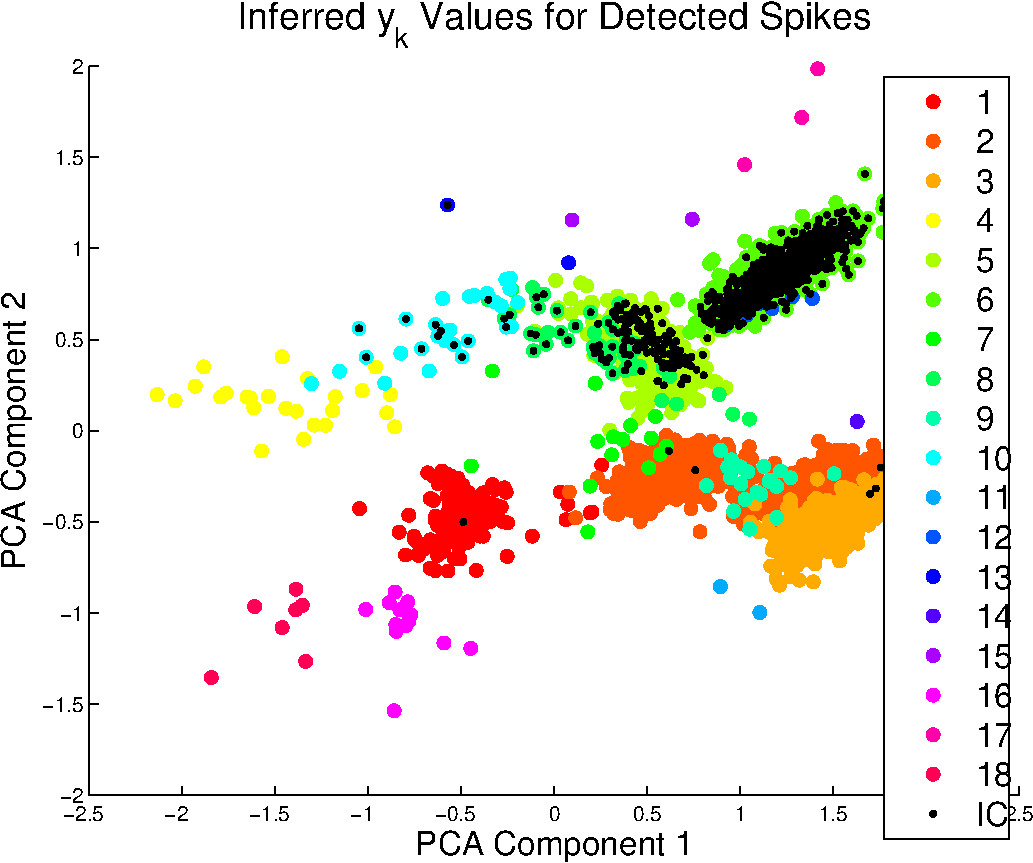
\includegraphics[width=\textwidth]{ykwn}
\caption{Inferred $y_t$ for detected spikes, online method with white noise model}
\end{figure}
\begin{figure}
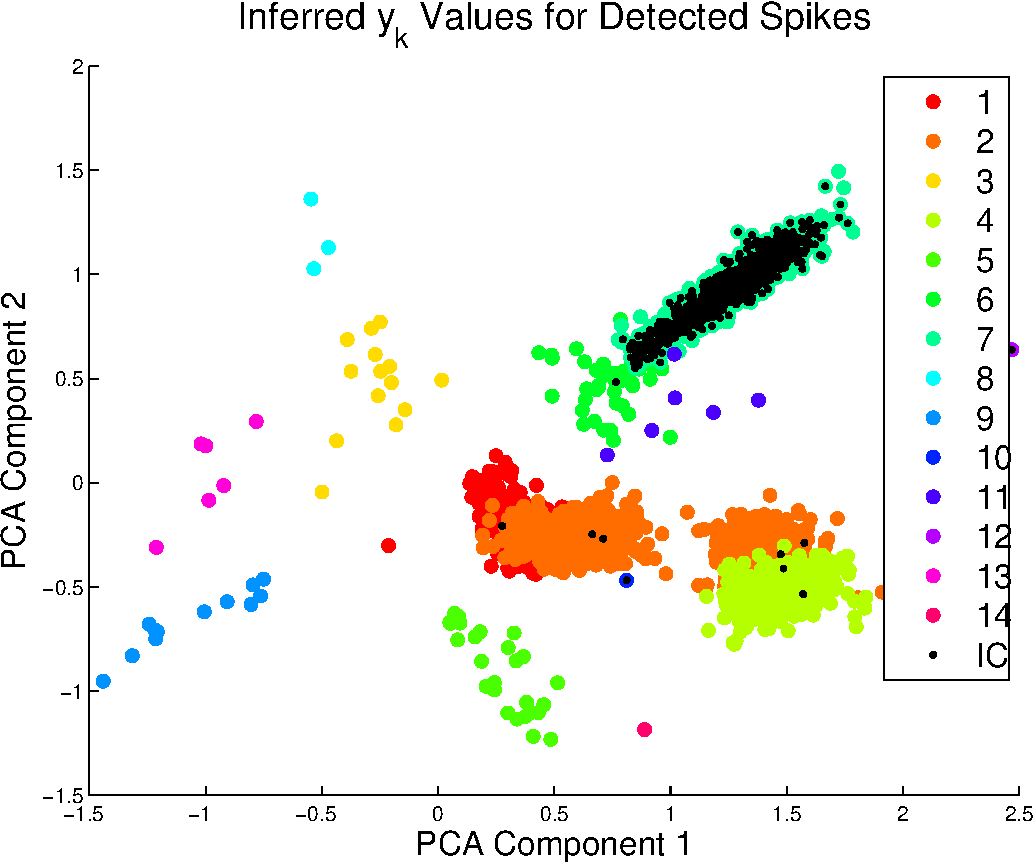
\includegraphics[width=\textwidth]{yk}
\caption{Inferred $y_t$ for detected spikes, online method with GP noise model}
\end{figure}
\begin{figure}
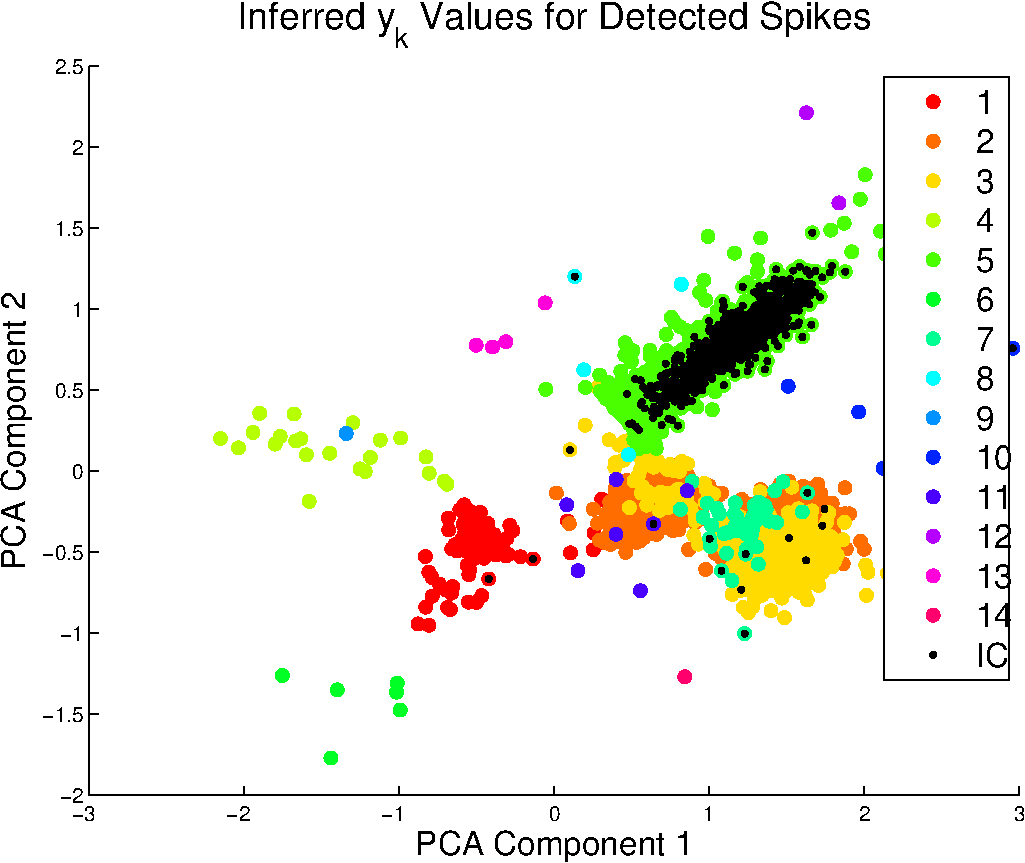
\includegraphics[width=\textwidth]{ykarwn}
\caption{Inferred $y_t$ for detected spikes, online method with GP mean with white noise model}
\end{figure}
\begin{figure}
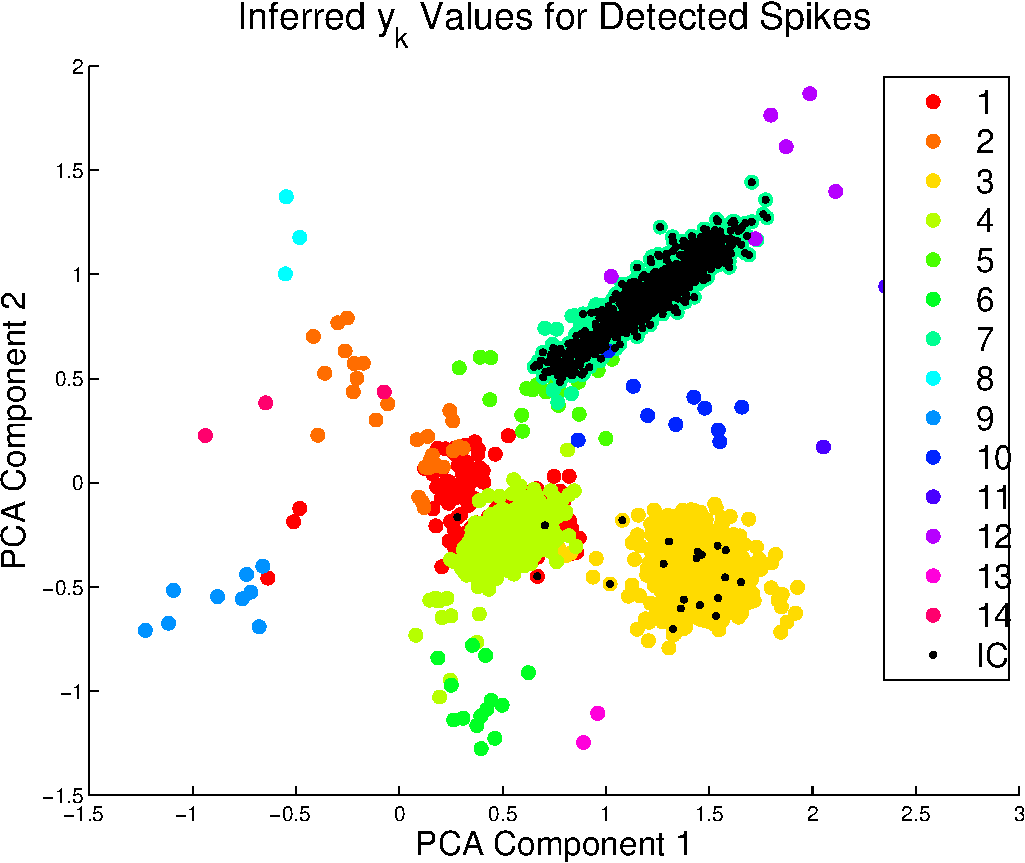
\includegraphics[width=\textwidth]{ykar}
\caption{Inferred $y_t$ for detected spikes, online method with GP mean and  GP noise model}
\end{figure}
\begin{figure}
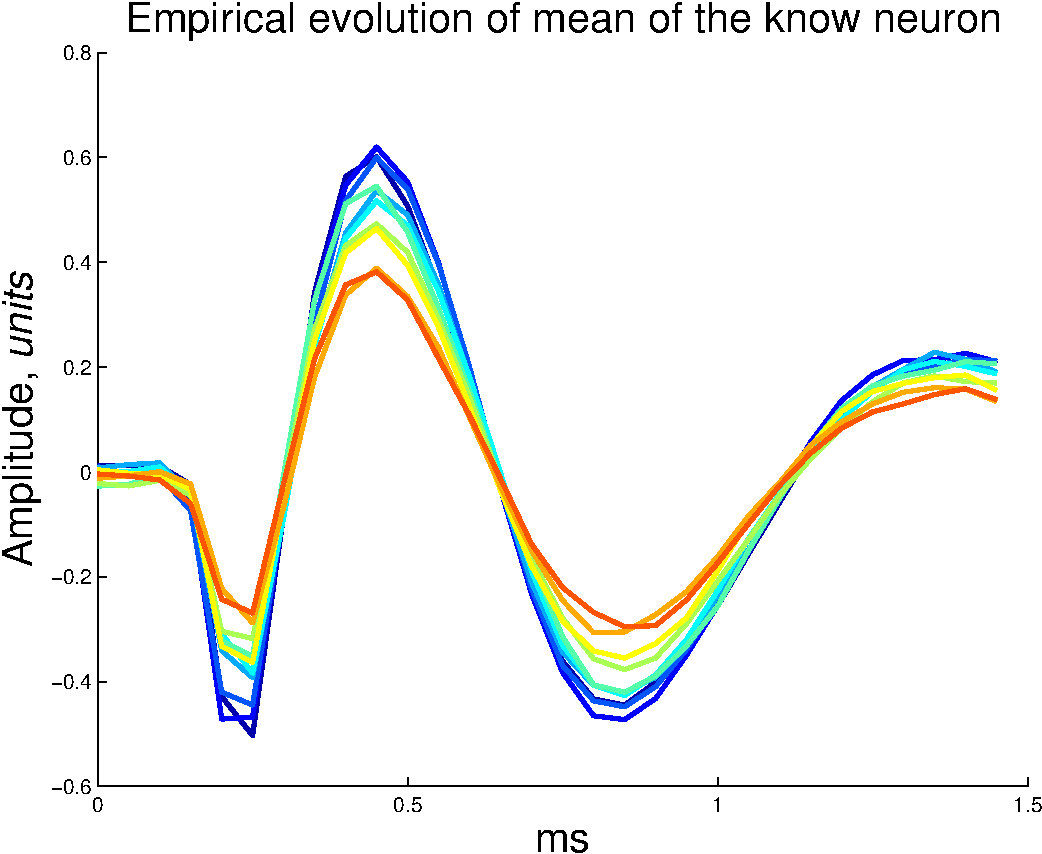
\includegraphics[width=\textwidth]{evohc1}
\caption{Mean of IC spikes over Time}
\end{figure}
\begin{figure}
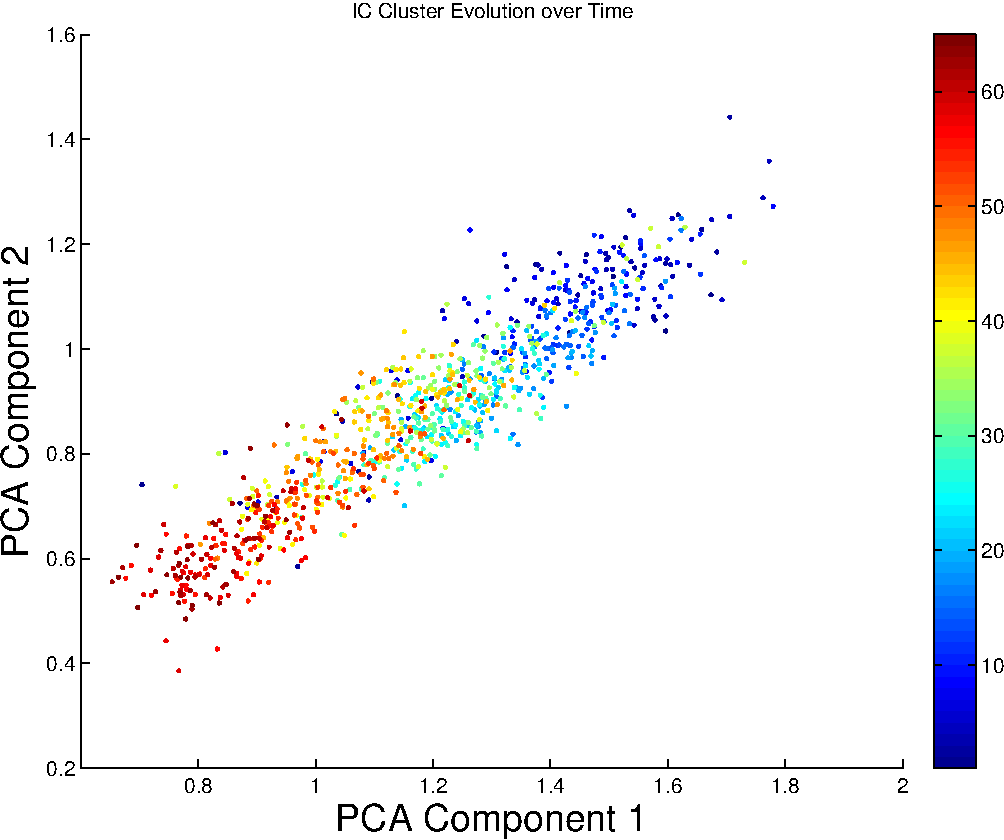
\includegraphics[width=\textwidth]{clusterevo}
\caption{Evolution of the IC cluster in the Online-GP mean and GP noise model}
\end{figure}
\begin{figure}
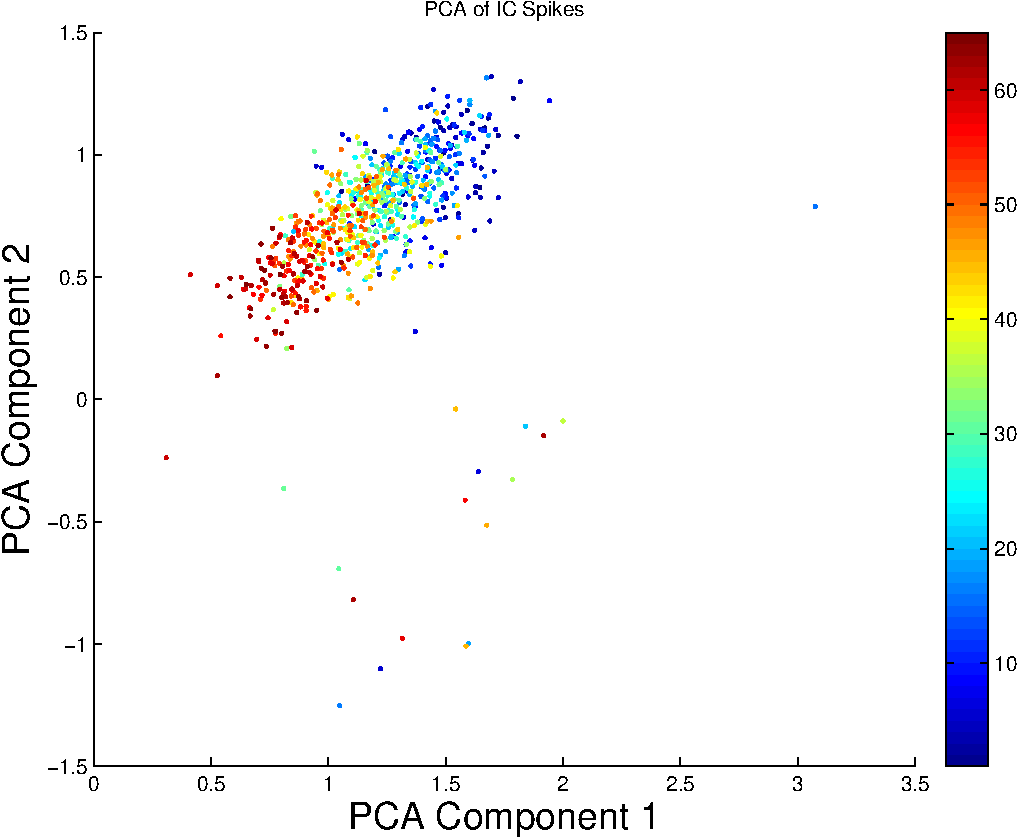
\includegraphics[width=\textwidth]{clustertrueevo}
\caption{PCA for IC spikes detected with thresholding}
\end{figure}

\end{document}




\section{Results}
I ran this on the full HC-1 dataset.  The algorithm found 11 clusters, with counts ( 1212, 1378, 26, 25, 97, 949, 3, 23, 8, 1, 3) and this corresponded to the following number of spikes from the intracellular neuron: (2, 6, 0, 0, 0, 807, 0, 0, 0, 0, 0, 0).  A spike in our dataset was considered to be associated with the intracellular neuron if the detected spike center was within 5 samples (.25ms) of the center of the intracellular spike.  This means that multiple spikes could get associated with the same intracellular spike if they were overlapping.  Using Qisong's error metric, this gives an "accuracy" of 95.70\% in total computation time of 32 (in highly unoptimized code!) seconds for the 2 minutes of data.  For the known cluster, we get that 85.04\% the spikes correspond to the known neuron.  Of the detected spikes associated with the known neuron, 97.94\% are in the same cluster.

There are at most 870 intracellular waveforms.  Using our method, we can detect at least 807 of them.  If we were to use the standard method of thresholding at 3x the standard deviation, 770 spikes were detected.  This is an increase of just under 5\%.  This

The PCA plot of the detected waveforms is shown below:
\begin{figure}
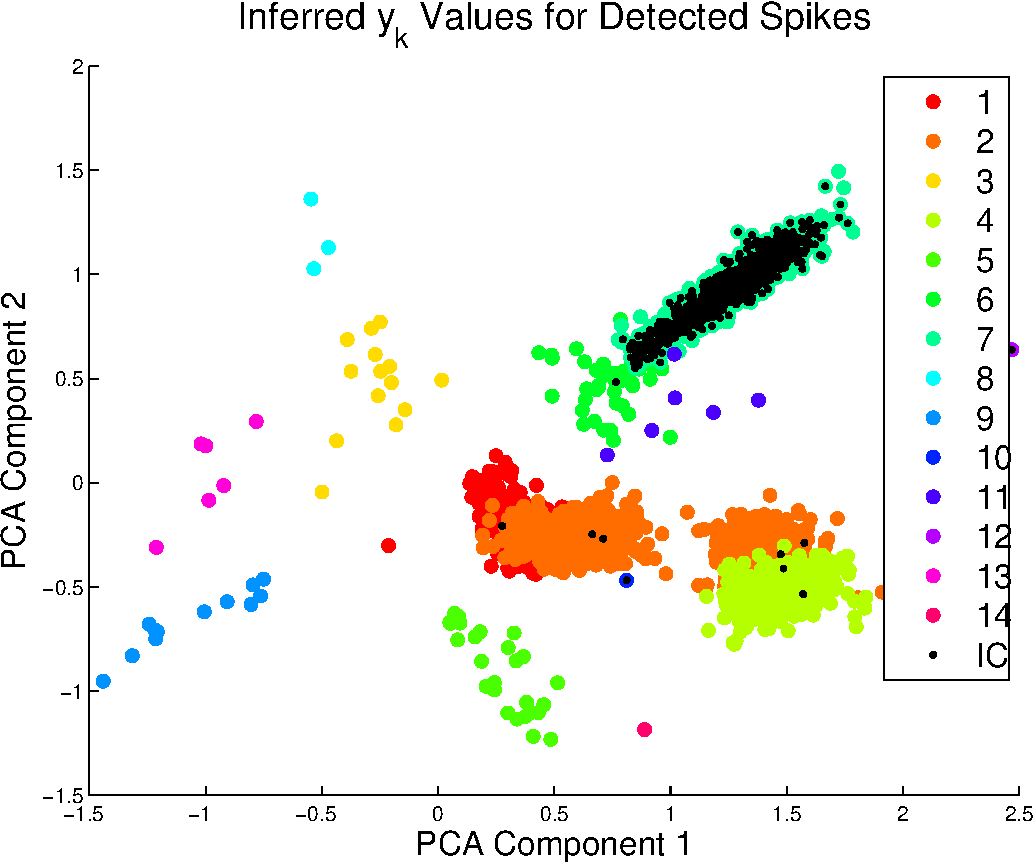
\includegraphics[width=\textwidth]{yk}
\caption{Detected Waveforms from the Online Method with AR(1) Noise Model}
\end{figure}
\begin{figure}
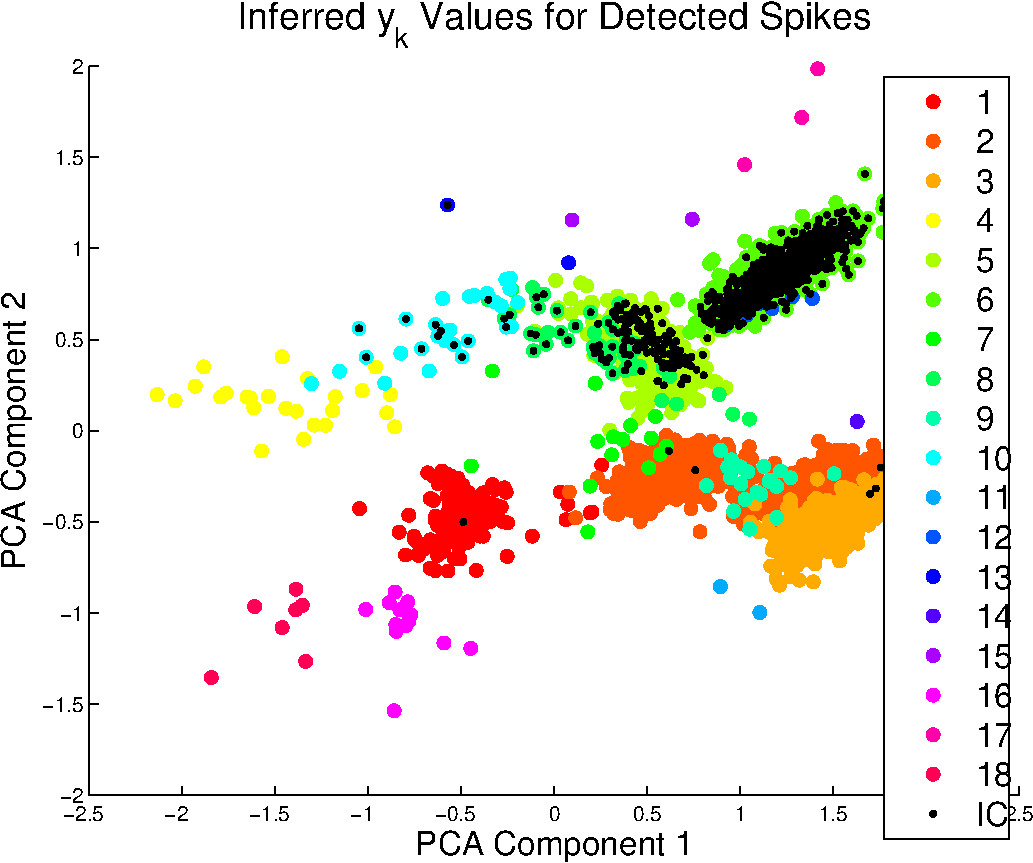
\includegraphics[width=\textwidth]{ykwn}
\caption{Detected Waveforms from the Online Method with White Noise Model}
\end{figure}








